\chapter{Các công trình liên quan}
\ifpdf
    \graphicspath{{Chapter2/Chapter2Figs/PNG/}{Chapter2/Chapter2Figs/PDF/}{Chapter2/Chapter2Figs/}}
\else
    \graphicspath{{Chapter2/Chapter2Figs/EPS/}{Chapter2/Chapter2Figs/}}
\fi

\paragraph*{}
Từ khi ra đời, bài toán phân lớp vật liệu nhận được sự chú ý của rất nhiều nhóm nghiên cứu. Cùng với sự phát triển đó, rất nhiều tập dữ liệu mới cũng được xây dưng để giải quyết nhiều vấn đề khác nhau của bài toán. Hình \ref{fig:timeline} là tóm tắt các công trình nghiên cứu liên quan được công bố tại hội nghị CVPR (Conference on Computer Vision and Pattern Recognition) từ năm 2010 tới nay. Bên cạnh đó bảng 2.1 là tổng hợp một số tập dữ liệu được sử dụng.

\begin{figure}[h!]
	\centering
	\captionsetup{width=0.9\textwidth}
	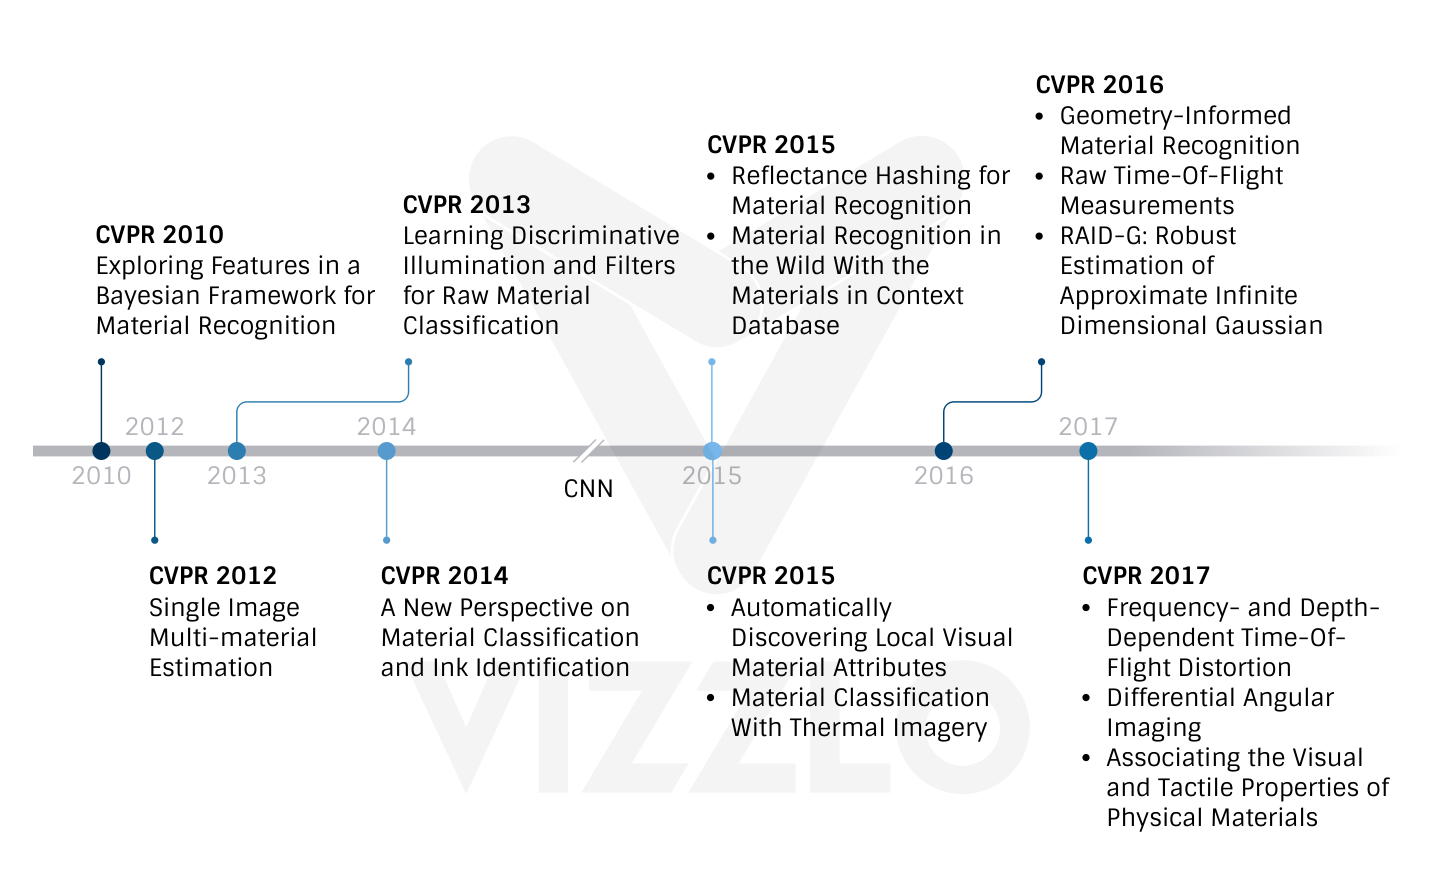
\includegraphics[width=1.0\textwidth]{timeline.png}
	\caption{Các nghiên cứu được công bố tại hội nghị CVPR qua các năm từ 2010 đến nay}
    \label{fig:timeline}
\end{figure}

\begin{table}
\label{tab:datasets}
\begin{center}
\resizebox{1.0\linewidth}{!}{
\begin{tabular}{l|l|l|l|l|l|l|l|l}
\toprule[1.0pt]
\head{Name}
& \head{Samples}
& \head{Classes}
& \head{Views}
& \head{Illumination}
& \head{In scene}
& \head{Scene image}
& \head{Camera parameters}
& \head{Year} \\
\midrule
CUReT \cite{dana1999reflectance} 				& 61	& 61	& 205	& 205 	& No	& No	& No	& 1999 	\\
KTH-TIPS \cite{hayman2004significance}			& 11	& 11	& 27	& 3		& No	& No	& No	& 2004	\\
UBO2014 \cite{weinmann2014material}				& 84	& 7		& 151	& 151	& No	& No	& No	& 2014	\\
Reflectance disk \cite{zhang2015reflectance}	& 190	& 19	& 3		& 3 	& No	& No	& Yes	& 2015	\\
4D Light-field \cite{wang20164d}				& 1200	& 12	& 1		& 1		& Yes	& No	& No	& 2016	\\
NISAR \cite{choe2016simultaneous} 				& 100	& 100	& 9		& 12	& No	& No	& No	& 2016	\\
GTOS \cite{xue2017differential} 				& 606	& 40	& 19	& 4		& Yes	& Yes	& Yes	& 2016 	\\
\bottomrule[1.0pt]
\end{tabular}}
\captionsetup{width=0.9\textwidth}
\caption{Một số tập dữ liệu được dùng cho phân lớp dữ liệu \cite{xue2017differential}}
\end{center}
\end{table}

\paragraph*{}
Một điểm chung có thể thấy, sau khi CNN bắt đầu được dùng nhiều trong Thị giác máy tính và chứng minh sự hiểu quả của chúng, số lượng và chất lượng của các nghiên cứu cũng tăng lên đáng kể (kết quả phân lớp rất chính xác, gần như bằng với khả năng đoán của con người), các tập dữ liệu được dùng cũng lớn hơn, đa dạng hơn.

\paragraph*{}
Có rất nhiều phương pháp khác nhau để giải quyết bài toán phân lớp vật liệu. Các phương pháp này có thể được chia thành hai nhóm chính: \textbf{Lab-based} và \textbf{Image-based}

\section{Lab-based methods}
\paragraph*{}
Đây là các phương pháp sử dụng chính các thông tin vật lý của đối tượng để phân lớp. Các thông tin vật lý có thể là độ đàn hồi (elasticity) \cite{davis2015visual}, sự thấm nước (water permeation) \cite{saponaro2015material}, phản ứng với ánh sáng (optical response) hay độ phản chiếu (reflectance) \cite{tanaka2017material}. Đây là các thông tin rất giá trị, vì vậy độ chính xác của các phương pháp này thường rất cao. Tuy nhiên quá trình xây dựng các bộ dữ liệu để thực hiện các phương pháp này rất kỳ công, đòi hỏi các thiết bị đặc biệt và một môi trường lý tưởng (vì vậy nên chúng có tên lab-based). Ví dụ, GelFabric \cite{yuan2017connecting} - tập dữ liệu ra đời năm 2016 chứa thông tin về chiều sâu và chỉ dùng để phân biệt các loại vải khác nhau; Ground Terrain in Outdoor Scenes (GTOS) \cite{xue2017differential} - năm 2016 dùng để lấy thông tin về các góc nhìn khác nhau cho cùng một mẫu trong dữ liệu; Reflectance Disk Database \cite{zhang2015reflectance} - năm 2015 với thông tin về sự phản chiếu của bề mặt. Thêm vào đó, các phương pháp khác nhau trong nhóm này thường đòi hỏi các thông tin vật lý khác nhau, chính vì thế tập dữ liệu của phương pháp khác nhau thường không thể dùng lại được. Ví dụ, một phương pháp dùng độ đàn hồi làm feature chính để phân lớp thì không thể dùng một tập dữ liệu chỉ có thông tin về độ thấm nước được. Vì vậy, các phương pháp đạt kết quả rất cao trên tập dữ liệu này có thể dễ dàng thất bại trên tập dữ liệu khác (hoặc không thể sử dụng trên dữ liệu khác vì thiếu thông tin). Hình \ref{fig:lab_based_1} và \ref{fig:lab_based_2} là hai ví dụ được lấy từ hai nghiên cứu năm 2017 và 2015 sử dụng các thông tin vật lý khác nhau (thông tin về chiều sâu, độ phản chiếu ánh sáng) để phân biệt các loại vật liệu. Cả hai đều đạt kết quả khá tốt trên những tập dữ liệu có đầy đủ thông tin trên \cite{tanaka2017material} \cite{zhang2015reflectance}

\begin{figure}[h!]
	\centering
	\captionsetup{width=0.9\textwidth}
	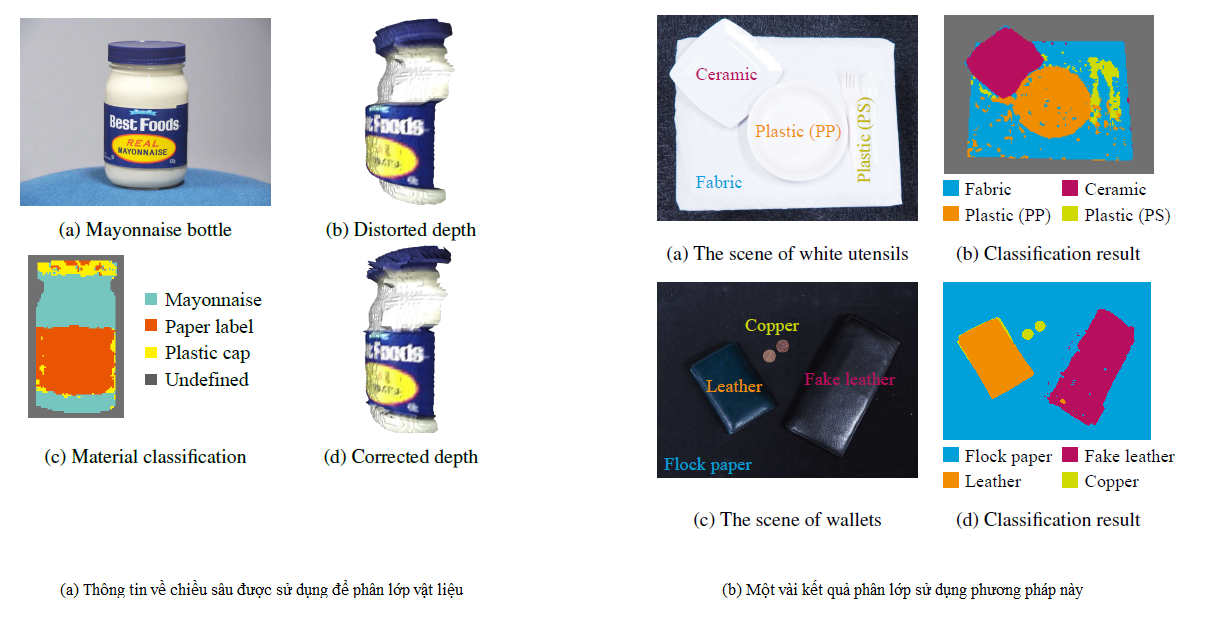
\includegraphics[width=1.0\textwidth]{lab_based_1.png}
	\caption{Thông tin về chiều sâu được dùng để phân lớp vật liệu trong một nghiên cứu 2017 \cite{tanaka2017material}}
    \label{fig:lab_based_1}
\end{figure}

\begin{figure}[h!]
	\centering
	\captionsetup{width=0.9\textwidth}
	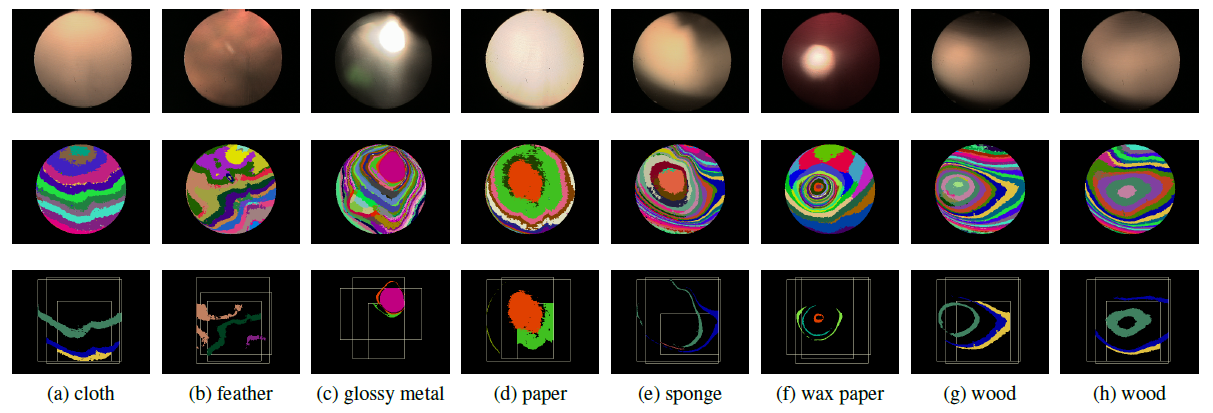
\includegraphics[width=1.0\textwidth]{lab_based_2.png}
	\caption{Thông tin về sự phản chiếu ánh sáng được dùng để phân lớp vật liệu trong một nghiên cứu 2015 \cite{zhang2015reflectance}}
    \label{fig:lab_based_2}
\end{figure}

\pagebreak

\section{Image-based methods}
\paragraph*{}
Ngược lại với các phương pháp Lab-base, Image-base là các phương pháp chỉ sử dụng ảnh màu RGB để phân lớp. Vì thế các tập dữ liệu cũng dễ dàng thu thập hơn, và các phương pháp này nếu có độ chính xác cao thì rất dễ để áp dụng vào thực tế. Dựa trên các thông tin trực quan (chẳng hạn như màu sắc) thông qua ảnh và thường dựa trên bài toán phân loại đối tượng để tìm ra vật liệu của ảnh (vì các phương pháp hiện tại dùng nhiều các mạng CNN được huấn luyện sẵn cho bài toán phân loại đối tượng để làm gốc), vấn đề chính của các hệ thống dùng phương pháp này chính là sự thiếu thông tin và vì thế chúng dễ dàng bị "lừa" bởi các ảnh có các đối tượng tương tự nhau nhưng lại khác nhau về chất liệu.
Hình \ref{fig:image_based_1} và \ref{fig:image_based_2} là hai ví dụ cho các phương pháp thuộc nhóm này được lấy từ các nghiên cứu năm 2010 \cite{liu2010exploring} và 2011 \cite{hu2011toward}. Trong những năm gần đây với sự phát triển của Deep Learning, các mạng CNN (Convolutional Neuron Network) được dùng thay thế cho các dạng local features này và nhiều nghiên cứu khác sử dụng các mạng CNN đã huấn luyện cho bài toán phân lớp đối tượng và đạt kết quả khá cao, tuy nhiên vẫn còn một số hạn chế như đã nêu bên trên. Nhóm tập trung giải quyết các hạn chế này và kế thừa các thành công từ CNN để cải thiện kết quả của bài toán.

\begin{figure}[h!]
	\centering
	\captionsetup{width=0.9\textwidth}
	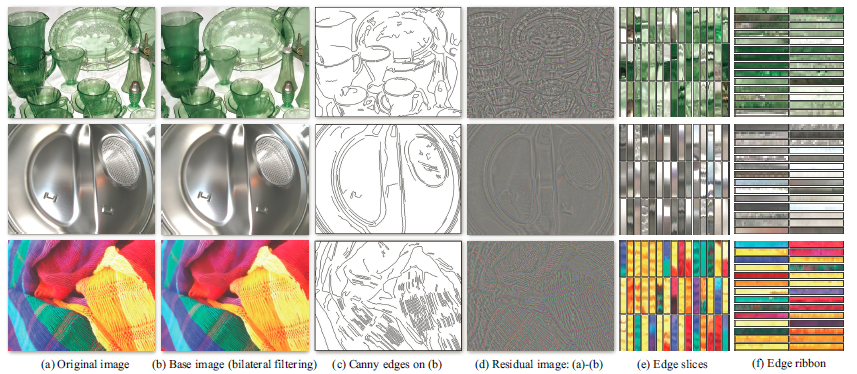
\includegraphics[width=1.0\textwidth]{image_based_1.png}
	\caption{Các local features (cạnh, \textit{micro structures}, SIFT - Scale-Invariant Feature Transform) được được dùng để phân lớp vật liệu trong một nghiên cứu 2010 \cite{liu2010exploring}}
    \label{fig:image_based_1}
\end{figure}

\begin{figure}[h!]
	\centering
	\captionsetup{width=0.9\textwidth}
	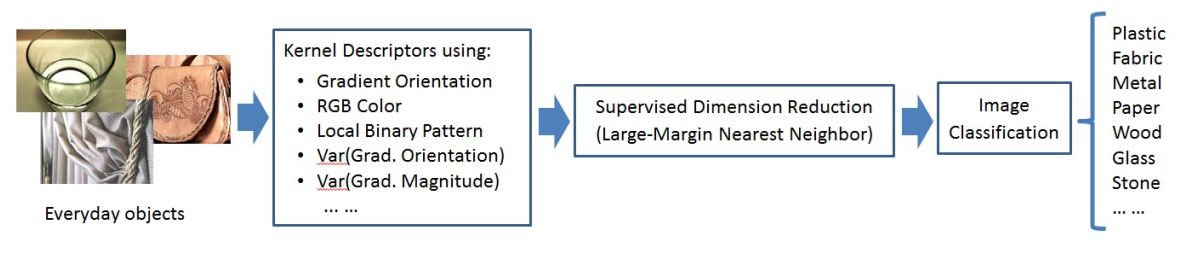
\includegraphics[width=1.0\textwidth]{image_based_2.png}
	\caption{Thông tin về gradient, màu sắc, local binary patterns được được dùng để phân lớp vật liệu trong một nghiên cứu 2011 \cite{hu2011toward}}
    \label{fig:image_based_2}
\end{figure}

\pagebreak
\paragraph*{}
Trong đề tài này, phương pháp mà nhóm sử dụng thuộc loại Image-based vì đối với lab-based, các tập dữ liệu sẽ được xậy dựng dựa trên phương pháp (đã có phương pháp X và xây dựng dữ liệu để phục vụ cho phương pháp X), cho nên các thông tin vật lý này dường như đã được sử dụng một cách triệt để nhất và nhóm sẽ có ít cơ hội hơn để cải tiến chúng. Ngoài ra, nhóm còn được thúc đẩy bởi một two-stream network (mạng với 2 nhánh chính) được dùng trên tập GTOS năm 2017\cite{xue2017differential}. Hình \ref{fig:dain} thể hiện ý tưởng chính của nghiên cứu này, sử dụng một hệ thống mạng CNN với hai nhánh đầu vào (một là ảnh gốc, hai là ảnh thể hiện thông tin khác nhau về góc nhìn (view-point) - hay được tác giả gọi là Differential Angular Image). Differential Angular Image được tạo thành bằng cách lấy hai ảnh của cùng một mẫu dữ liệu được chụp từ hai góc khác nhau (hai góc này chênh lệch không quá nhiều) trừ nhau (Hình \ref{fig:differential_angular}). 

\begin{figure}[h!]
	\centering
	\captionsetup{width=0.9\textwidth}
	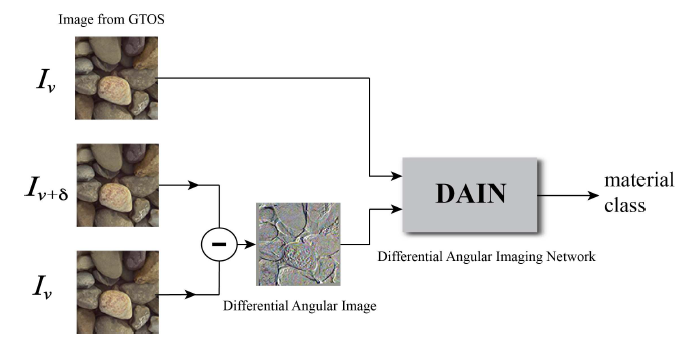
\includegraphics[width=1.0\textwidth]{dain.PNG}
	\caption{Two-stream network được dùng trên tập GTOS năm 2017 \cite{xue2017differential}}
    \label{fig:dain}
\end{figure}

\begin{figure}[h!]
	\centering
	\captionsetup{width=0.9\textwidth}
	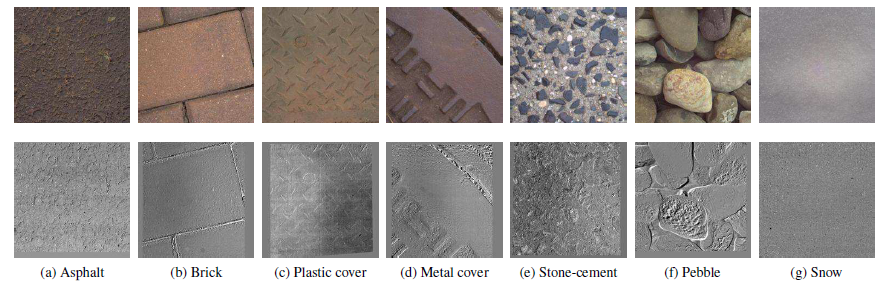
\includegraphics[width=1.0\textwidth]{diferential_angular.png}
	\caption{Differential Angular Image được tạo thành bằng cách lấy hai ảnh của cùng một mẫu dữ liệu được chụp từ hai góc khác nhau (hai góc này chênh lệch không quá nhiều) trừ nhau \cite{xue2017differential}}
    \label{fig:differential_angular}
\end{figure}

\begin{figure}[h!]
	\centering
	\captionsetup{width=0.9\textwidth}
	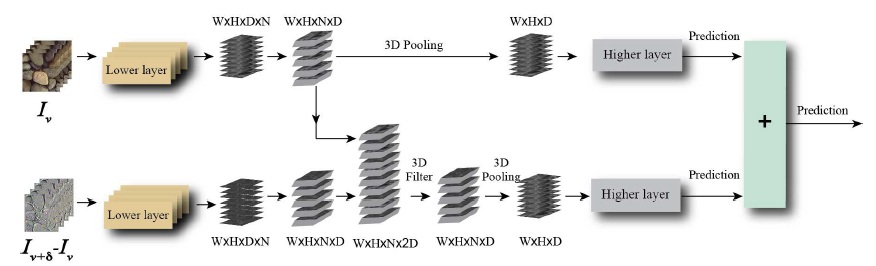
\includegraphics[width=1.0\textwidth]{dain_network.png}
	\caption{Cấu trúc bên trong của DAIN (Differential Angular Image Network) \cite{xue2017differential}}
    \label{fig:dain_network}
\end{figure}
